\documentclass[titlepage]{article}
\usepackage{graphicx}
\usepackage{pdfpages}
\usepackage{longtable}
\usepackage{tabu}

\title{The Undecided - Final Report - 7CCSMGRP}
\author{Nathalie Caliacmani, Amar Menezes, \\ Belema Norman-William, Paul Orlean-Taub, Tony Sellen}
\date{March 2015}

\begin{document}

\includepdf[pages={1,2}]{CoverSheet.pdf}
\maketitle

\begin{abstract}
Since its development, the car has had a huge economic and social influence. It has created industries and caused others to crumble. The popularity of the auto-mobile has had an impact on city planning due to its effects on employment, trade, manufacture and even basic social interaction.

As the popularity of these vehicles in both a private and public context has increased, transport planners and civil engineers have had to adjust our road networks accordingly often through the development of mathematical models for traffic flow (of varying accuracy).

This project is our attempt at producing a software  package that shows the effects of changes to pre-existing networks (i.e. increase/decrease in demand, adding lanes, changing existing lanes into bus lanes) on the overall flow. The primary output will be data that can be fed into an appropriate statistical package for professional analysis.
\end{abstract}

\tableofcontents
\newpage

\section{Introduction}
		In 1769, Cugnot developed the first steam powered auto-mobile \cite{eckermann2001world} (self propelled vehicle not operating on tracks). As these vehicles spread to the UK, the government passed the locomotive acts providing a framework for the automotive industry here to develop and regulating the use of these machines; The act of 1861 imposed speed limits, determined tolls, set fines, and stated design requirements; the act of 1865 tightened these regulations and required that a man waving a red flag would be required to walk ahead of all of these vehicles; and the 1878 act assigning the powers.
	
	In 1886\footnote{The same year Coca Cola was invented} Karl Benz filed his patent for the petrol powered ``moterwagen'' \cite{benzpatent} sparking the production of uniform vehicles that could travel long distances. The uptake of these machines leading to further regulations and the requirement for licensing. From this time onwards there was a steady increase in car ownership, primarily amongst the wealthy and private businesses.

	In 1908, the Ford Motor Company developed the Ford Model T, and with it, the automatic assembly line allowing the production of these cars in 93 minutes. The increase in production speed allowed costs to be optimised and made the car affordable to the mass market.
	
	In the years that followed, cars became a primary mode of transportation. In response to increased usage, the British government passed laws that were less restrictive on car use, and optimised road networks to cope with an increase in vehicles that were larger, heavier, and faster than those for which they were originally developed.
	
	Nowadays cars are widespread, and finely engrained in our culture\cite{miller2001car}\cite{berdahl2000go}. However new developments lead to large changes in ownership rates and road demand, and many economies rely on the optimisation of traffic flow, with traffic engineers often needing to change factors in order to artificially increase and decrease congestion \cite{blunden1983congestion}. These engineers use mathematical models to simulate flow through a network and often need to trial the effects of various changes.
	
	This project is our attempt at producing a piece of software to model a road network and create artificial (and hopefully realistic) data that will allow a civil engineer to perform the appropriate analysis and determine the best way to optimise our pre-set systems 

\section{Review}
	\subsection{Overview}
	Computer simulation is getting popular in the field of science. Individuals tackle diverse experimental issues using computer control through simulating artificial testing environments. They use these simulated environments to test scientific models in order to prove or disprove their feasibility and correctness.
	 
	Today's high machine power gives people the capacity to simulate environments at a rate much quicker than any real environment, thus any experiment carried out in the simulated medium would provide results minutes, hours, days and often weeks, months and years ahead of what the same experiment would provide if executed in the real world.
	
	One of the frameworks or systems that are best considered using a computer simulation is a traffic network. It is typical to experiment with traffic networks in a computer-simulated environment because experimenting with traffic in the real environment is impractical. 

\subsection{Simulation models}
	A typical classification method for simulation models is based on the variability content that represents the deterministic nature of simulation that represents the static or dynamic characteristics of simulation. Regarding how frequent the activity of the traffic network is updated and the statistics on traffic performance is collected, the most frequently used classification method is based on the details a model intends to simulate, namely, microscopic or macroscopic modelling.
\subsubsection{Microscopic modelling}
	Microscopic simulation modeling methods are based on car-following and lane-changing theories, which can represent the traffic operations and vehicle/driver behaviors in detail. The car-following theory describes the longitudinal movement of vehicles. The classical car-following approach is quite straightforward, i.e., each vehicle attempts to advance at its desired speed while maintaining a safe following distance from the vehicle ahead. [4] Microscopic simulation modelling incorporates queuing analysis, shock-wave analysis, and other analytical techniques.
\subsubsection{Macroscopic modelling}
	Macroscopic models do not consider car-following behaviour in detail, but instead model traffic as an aggregate fluid flow. To better understand the collective behaviour of traffic and analyse flow conditions in a dynamic fashion, continuum models, either simple or high-order, are usually employed in macroscopic simulation modelling. The simple continuum model consists of a continuity equation representing the relationship between the speed, density, and flow generation rate. [5] Although the existing high-order models look promising, they have not as yet proved truly superior to the simple continuum models at least in medium-to-congested flow conditions [6]
\subsection{Comparison of different traffic simulation packages}
	We will briefly review the following well known and widely used simulation packages;
	
	\begin{itemize}
		\item Simulation of Urban Mobility (SUMO)
		\item Quadstone Paramics Modeller
		\item Aimsun
	\end{itemize}

\subsubsection{Simulation of Urban Mobility (SUMO)}
	Simulation of Urban Mobility (SUMO) is an open source, very compact, microscopic road traffic simulation package designed to handle large road networks. [1]
	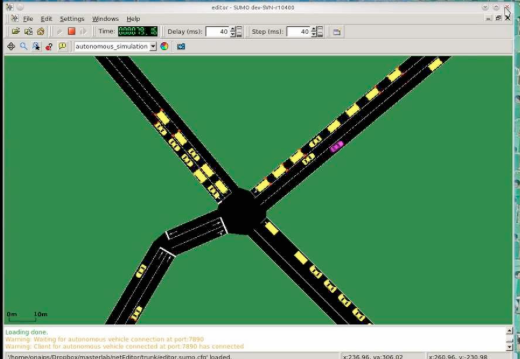
\includegraphics[scale=0.7]{./images/SUMO.png}
	The simulation platform SUMO's features include:
	\begin{itemize}
		\item Microscopic simulation – vehicles and public transport are modelled explicitly.
		\item Simulation of multi-modal traffic, e.g., vehicles, public transport and pedestrians.
	\end{itemize}

	
\section{Requirements and Design}
	The following is extracted from our initial report \cite{init}
\subsection{Objectives}
	Our primary objective is to create a system which can take as input a road system
	and a journey matrix and produce overall statistics about journey times between the entry/exit points
	and allow us to change something about the network or the demand and produce new statistics for
	comparison. Our aim is to model individual vehicle movements as realistically as possible, taking 
	into account driver type, vehicle type, car following behaviour, lane switching behaviour and junction
	modelling. The system will output statistics and raw data for each vehicle journey which could be
	further analysed using a statistical analysis tool such as SPSS.
\\ \\
	\subsection{Project Roadmap}
	
	\begin{description}
		\item[Stage 1] Decide on a model for traffic simulation.
		\item[Stage 2] Research existing implementations.
		\item[Stage 3] Develop architecture for the system(see \ref{secarch}).
		\item[Stage 4] Decide on a development methodology and technology to build the system.
		\item[Stage 5] Build the Core. The Core consists of the building blocks of the simulation i.e. Roads, Junctions, Vehicles.
		\item[Stage 6] Build Services around the Core. Services control the running of simulation, traffic light scheduling, populating the demand matrix, gathering and reporting statistics.  
		\item[Stage 7] Build a Client. The Client is a User Interface to the system. The Client allows the user to access system services.
		\item[Stage 8] Final report.
		\\
	\end{description}
	
	\subsection{Design}
		\label{secarch}
	The Core of the system consists of the following entities
	\begin{enumerate}
		\item Vehicle: This describes an entity travelling on the network. Vehicles have speed, acceleration, a maximum speed and behaviour. The vehicle is configured with a Source node and Destination node when it's added to the simulation. 
		
		\item Node: A node is the base component of our road model. A node represents a cell in the cell automata model. Each node can accommodate a vehicle of length one. A sequence of nodes forms a lane.
		
		\item Lane: A lane is a sequence of nodes that represents a lane on a road. Each lane supports traffic in one direction.
		
		\item Road: A road is comprised of one or more lanes. They allow travel in one direction, from a source, to a sink.
		
		\item Junctions: Junctions allow for transferring traffic between two or more road segments. In our base model we will allow each junction to have four interfaces (North, East, South \& West). Each interface has a junction entry and an exit mapping onto roads to build the network.
	\end{enumerate}
	The Services provided by the system are as follows
	\begin{enumerate}
		\item Control the running of the simulation by modifying the tick of the global clock.
		
		\item Configure the schedule of the traffic signals at the different junctions.
		
		\item Populate the Demand Matrix which specifies the density of traffic between two destinations.
		
		\item Mechanism to gather statistics on average journey time, average speed, etc.
	\end{enumerate}
	
	\subsubsection{Routing configuration}
		Each junction maintains a routing table to move vehicles to the appropriate junction exit towards their destination. These routing tables will be initially static, but may be made to function dynamically as we increase the sophistication of our network.
		
	\subsubsection{Policy configuration}
	
	\begin{enumerate}
		\item The user can supply a demand matrix to the simulation. This demand matrix will determine the relative frequency of vehicles travelling between any two destinations. A multiplier will then be calculated using other available information to determine the absolute values.
		\item The user can control the scheduling of traffic signals at junctions.
	\end{enumerate}
    \subsection{UML}
    \subsubsection{Use case diagram}
    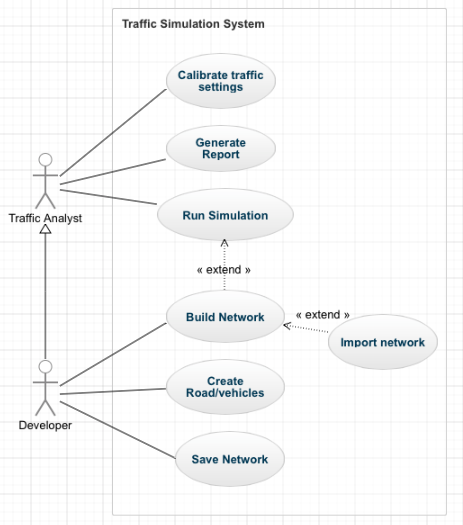
\includegraphics[scale=0.7]{./images/usecase.png}
    
    
\textit{Run Simulation} \\
The Traffic analyst chooses to run the simulation. The system starts the simulation and provides visual feedback while it is running. The traffic analyst can stop or start the simulation whenever he/she decides to do. When the traffic analyst decides to stop the simulation the, system stops running the simulation and keeps the model in this state, allowing the traffic analyst to subsequently start or run the simulation from where it was stopped.\\


\textit{Calibrate Traffic settings} \\
The Traffic analyst or developer chooses to adjust the traffic settings. The system displays available settings to change. Using the graphical interface widgets, the traffic analyst or developer can alters any traffic settings such as; traffic light interval, maximum velocity of vehicles, clock interval, the demand matrix for cars and buses. The system stores the new values of any adjustments or changes made. \\

\textit{Generate report} \\
The traffic analyst chooses to generate a report of the simulation. The system generates the report with all recorded statistics in text format. \\

\textit{Build New Network} \\
The developer chooses to build a new network. The system creates a blank network or alternatively, the developer can choose to Import Network. The system is now ready for another network simulation and calibrating traffic settings. \\

\textit{Create Road/Vehicles} \\
The developer creates new road and lanes, junctions, roundabouts on the network and different vehicles either cars or bus. \\

\textit{Import Network} \\
The system provides a file chooser. The developer finds an existing traffic network file saved on his/her device. The system verifies and loads the existing network into the model. \\

\textit{Save Network} \\
The developer chooses to save the network to the model. The system provides a file chooser to determine where to save. The developer selects an existing file or gives a name for a new network file.\\
 \subsubsection{class diagram}
Road Network class design with vehicle class\\
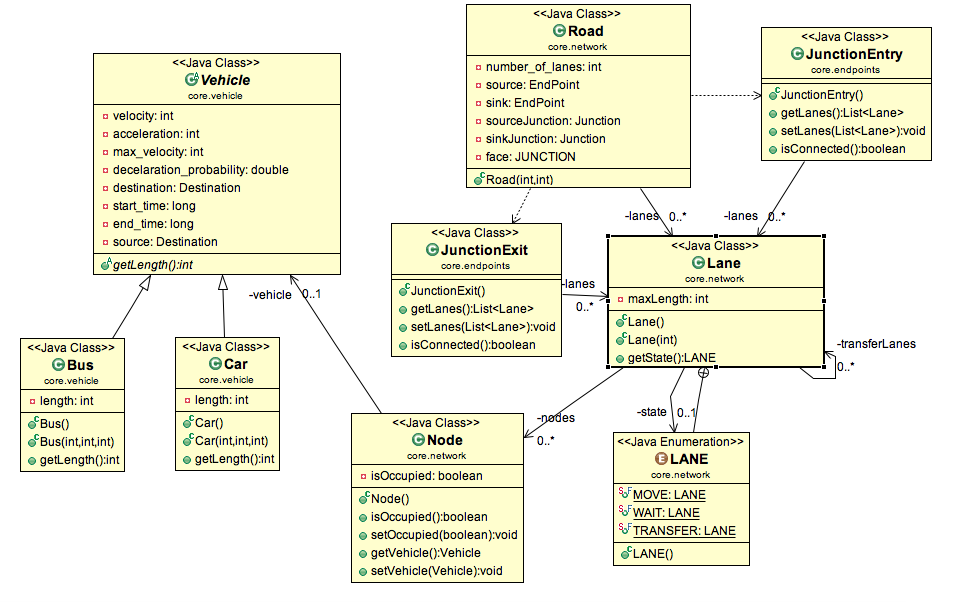
\includegraphics[scale=0.3]{./images/class1.png} ~\\

The above diagram shows the traffic network using links and nodes, the system represents the road on a discrete network of cells, the roads can be vertical, horizontal or even both. It allows different scenarios to be modelled. A junction is simply a road with lanes leading to it in different direction. In this model there are two types of vehicles namely; buses and cars.

\subsubsection{Traffic lights and junctions}
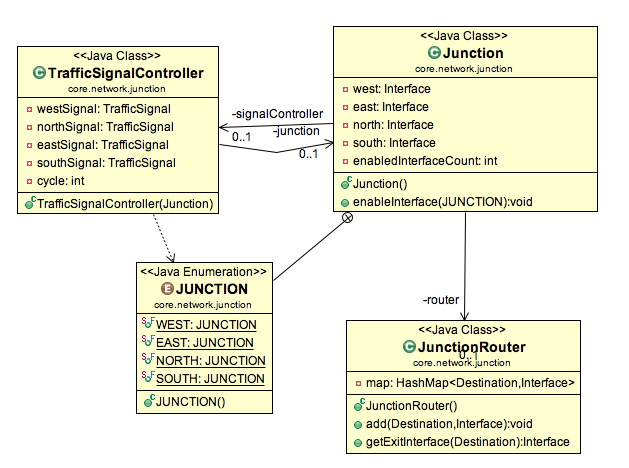
\includegraphics[scale=0.4]{./images/class4.png}


The class diagram above shows the relationship between the traffic signal controller and the junctions in all four directions; north, south, east and west. This function defines the basis of the network, as the vehicles will follow the instructions given by the traffic signal control at each junction in order to safely get to their various destinations

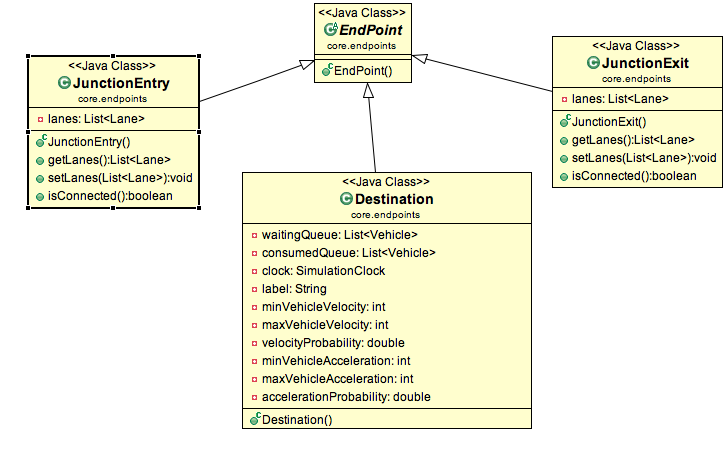
\includegraphics[scale=0.4]{./images/class3.png}

\subsubsection{Sequence Diagram}

Sequence diagrams are sorts of interaction diagram that show the flow of messages through a framework as a specific function is being executed. The sequence diagram below describes the sequence of events that occur during a simulation run. It shows a single interval, and during normal use, this sequence would be repeated for the duration of the simulation. \\
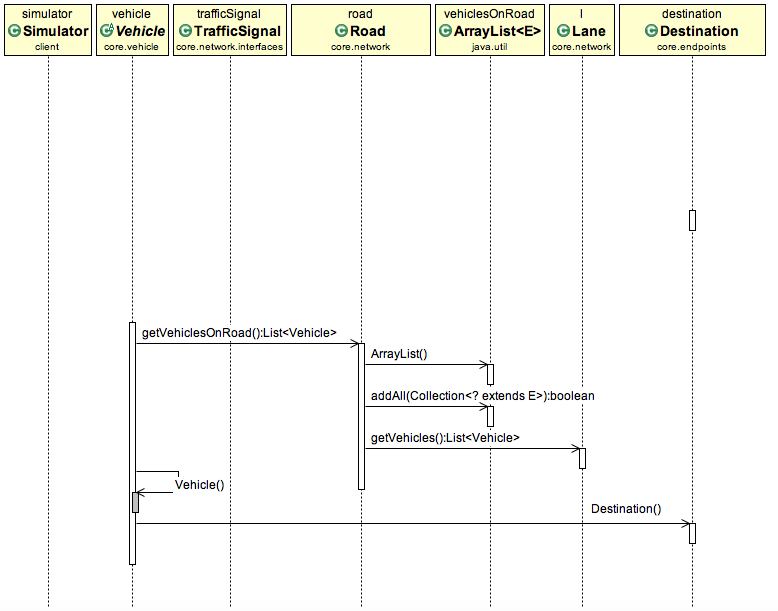
\includegraphics[scale=0.4]{./images/interaction.png}








	
\section{Implementation}
	\subsection{Output}
We designed the software to output individual car journeys for a transport consultant to analyse using statistical analysis packages.  The basic idea is that the software is used to support decisions about  changes to the road network or for supporting planning decisions.  We present two scenarios here. Instead of using a statistical analysis package such as SPSS we wrote a custom python script to summarise the data.  The script also serves as a sanity check for the output of our software.  The python script is included in the appendix to this report. 



\subsubsection{Shopping Centre Development}
We have a simple network as shown below.  The consultant does a survey to measure existing traffic movements which we translate into a \textit{demand matrix} for the road system.  The demand matrix is just a count of car movements between each end point of the network over a given time period.  We are keeping things simple in our example and only considering one vehicle type.  In reality the model would take into account of other vehicle types and our software does allow for that.  We convert this demand matrix into a table which specifies the probability of a car entering the network at for each combination of origin and destination for each tick of the simulation clock.  This drives the creation of vehicles in our simulation for the base case.  \\ The consultant runs other models, based on the size of the new shopping centre and proximity of other centres to estimate a new demand matrix for when the centre is built.  Our software is then run in the base case and the modelled case using the new demand matrix and reports are generated showing the effect on journey times.\\ \textbf{Network diagram}
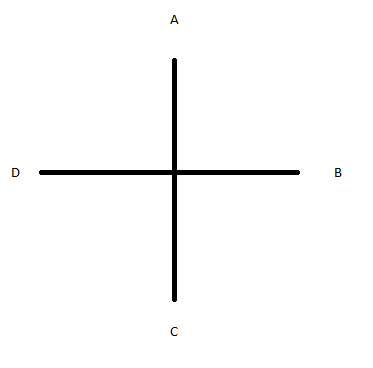
\includegraphics[scale=0.5]{./images/network.png}

We used the following trip matrix for the base case:
	\begin{center}
	\begin{tabular}{| c | c | c | c | c |}
		\hline
		\textbf{ }	&	A & B & C & D \\ \hline
		A				&	0 & 0.3 & 0.3 & 0.3				\\ \hline
		B					&	0.3 & 0 & 0.3 & 0.3				\\ \hline
		C	&	0.3 & 0.3 & 0 & 0.3			\\ \hline
		D				&	0.3 & 0.3 & 0.3 & 0				\\ \hline

		
	\end{tabular}
	\end{center} and the following matrix, showing extra demand to and from the shopping centre at C
    \begin{center}
	\begin{tabular}{| c | c | c | c | c |}
		\hline
		\textbf{ }	&	A & B & C & D \\ \hline
		A				&	0 & 0.3 & 0.8 & 0.3				\\ \hline
		B					&	0.3 & 0 & 0.8 & 0.3				\\ \hline
		C	&	0.5 & 0.5 & 0 & 0.5			\\ \hline
		D				&	0.3 & 0.3 & 0.8 & 0				\\ \hline

		
	\end{tabular}
	\end{center}
    
    The output shows the expected behaviour:  proportionally more cars going to and from C and the average journey times to C increased.  The output for the two cases is shown below\\ \textbf{Base case}\\
    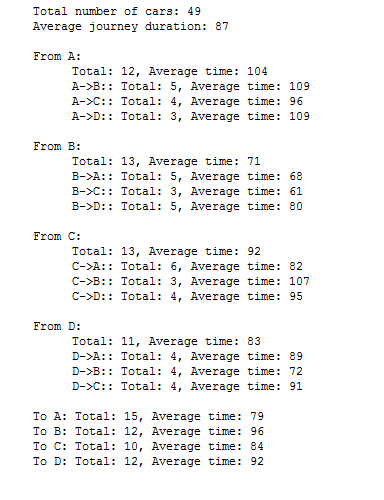
\includegraphics[scale=1.0]{./images/scenario1.png}\\ \textbf{Planned Shopping Centre}\\
    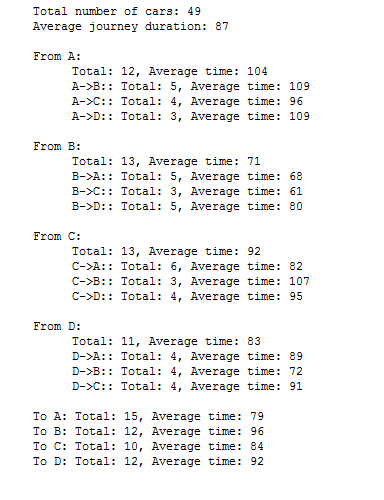
\includegraphics[scale=1.0]{./images/scenario2.png}
    
    
\subsubsection{Congestion Charge}
This scenario is similar to the Shopping Centre example but this time we are reducing demand for journeys to one node in the network by introducing a toll in the road system.  We should see a reduction in journey times as congestion is reduced.
   
    

In this case we used the following trip matrix and got the output below, which supports the case for a congestion charge at C reducing journey times
 \begin{center}
	\begin{tabular}{| c | c | c | c | c |}
		\hline
		\textbf{ }	&	A & B & C & D \\ \hline
		A				&	0 & 0.5 & 0.1 & 0.3				\\ \hline
		B					&	0.3 & 0 & 0.1 & 0.3				\\ \hline
		C	&	0.3 & 0.3 & 0 & 0.3			\\ \hline
		D				&	0.3 & 0.5 & 0.1 & 0				\\ \hline

		
	\end{tabular}
	\end{center}
~ \\ \textbf{Planned Shopping Centre}\\
    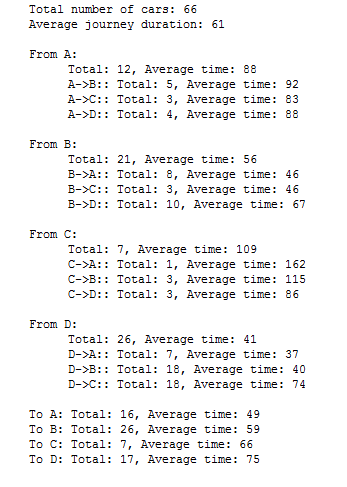
\includegraphics[scale=1.0]{./images/scenario3.png}

\section{Teamwork}
	We started out by assessing the skills of each team member and breaking down the task into smaller sub tasks.  We then made an initial allocation of team members to sub tasks based on our assessment of matching skills to the tasks.

On a day-to-day basis we tracked the progress of the project by using an online task and project management web system called Agilefant. 

Agilefant allows one to set up projects, assign team members, break the project down into major tasks and split the tasks down into smaller sub tasks and set up dependencies between the small tasks.

In our case we broke the software down into “core”, “client” and “services” and initially allocated at most two team members to each section.  As time progressed, based on how quickly we were getting different sections done and depending on if there were dependencies which needed to be worked on, we moved people around and reallocated tasks.


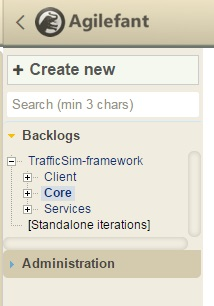
\includegraphics[scale=0.7]{./images/menu.jpg}

Agilefant allowed us to see at a glance how the small tasks within each of the major subtasks was going and how we were progressing towards our target.  It also alerted us to any dependencies which needed doing urgently and helped us make decisions about moving team members onto different tasks. \\
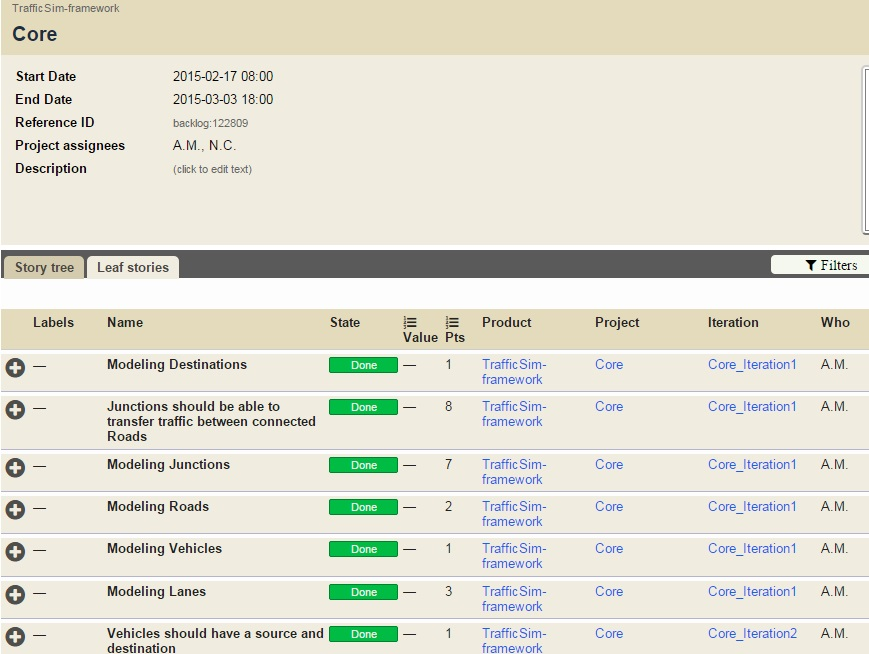
\includegraphics[scale=0.5]{./images/tasks.jpg}

The “burnup” chart shows completed tasks in green against the total scope of the sub-project. 
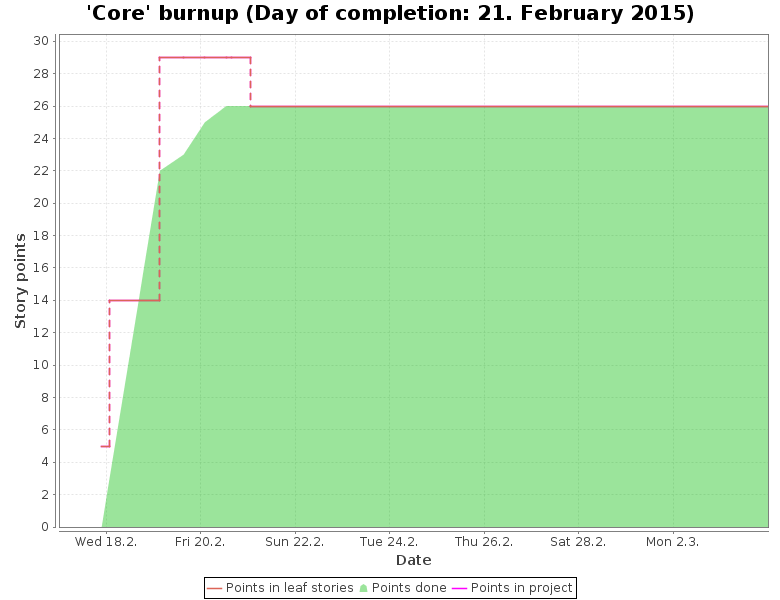
\includegraphics[scale=0.3]{./images/burnup_chart.png}

Dependencies can be clearly identified \\
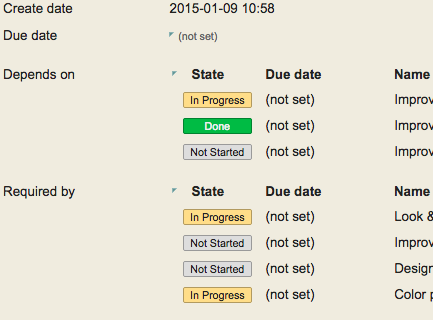
\includegraphics[]{./images/dependencies.png}

The sub-teams for the sub-projects core, client and services each consisted of one or more team member(s) at any one time.  There was overlap as any team member might be in more than one sub-team at any one time.  We allocated one person to be the team leader for each sub team at any one time.  The team leader was responsible for allocating tasks within the sub-team and also for identifying any problems and dependencies.  The sub-teams worked independently from each other and could organise their own meetings or ways of working as they saw fit.

We had weekly whole team progress meetings to evaluate how each sub-team was performing and discuss any necessary changes to the overall structure of the group or of the project. The team leaders for each sub-team reported to the whole group and made recommendations about resourcing which were discussed and agreed upon at the meeting.  Any changes agreed were recorded and subsequently emailed to all team members.
\section{Evaluation}
	%Critically evaluate your project: what worked well, and what didn't? how
%did you do relative to your plan? what changes were the result of improved thinking
%and what changes were forced upon you? how did your team work together? etc. Note
%that you need to show that you understand the weaknesses in your work as well as its
%strengths. You may wish to identify relevant future work that could be done on your
%project.
	\subsection{Initial aims}
	\subsection{Changes}
	\subsection{Possible improvements}
	\subsection{Future work}
		As a group we discussed ways we would improve this project 

\section{Peer Assessment}
	\begin{center}
	\begin{tabular}{| l | c |}
		\hline
		\textbf{Name}					&	\textbf{Points} \\ \hline
		Nathalie Caliacmani				&	20				\\ \hline
		Amar Menezes					&	20				\\ \hline
		Belema (Emily) Norman-William	&	20				\\ \hline
		Paul Orlean-Taub				&	20				\\ \hline
		Anthony Sellen					&	20				\\ \hline
		\textbf{Sum}					&	\textbf{100}	\\
		\hline
	\end{tabular}
	\end{center}
	
\bibliographystyle{plain}
\bibliography{./files/bibfile}

\appendix
\section{Git log}
\begin{center}
\begin{longtabu} to \textwidth {|
    X[4,l]|
    X[3,c]|
    X[8,l]|}
    \hline
    \textbf{Author} & \textbf{Date} & \textbf{Message} \ \hline
Amar Menezes & 2015-01-28 & Initial commit \\ \hline
Amar Menezes & 2015-01-28 & Updated Readme \\ \hline
Amar Menezes & 2015-01-28 & Initial Import \\ \hline
Amar Menezes & 2015-01-28 & Created Lane model to simulate a road \\ \hline
Amar Menezes & 2015-01-28 & Fixed OutOfBounds bug when cars exited the lane \\ \hline
Amar Menezes & 2015-01-29 & Cleaned up Main.java \\ \hline
Amar Menezes & 2015-01-29 & Fixed CarJump bug \\ \hline
Amar Menezes & 2015-01-29 & Cleared unused data structures \\ \hline
Amar Menezes & 2015-01-30 & Fixed CarJump bug when variable car speeds are used \\ \hline
Amar Menezes & 2015-01-31 & Added car acceleration \\ \hline
Amar Menezes & 2015-02-01 & Added unit tests \\ \hline
Amar Menezes & 2015-02-01 & Added tests for lane leaving \\ \hline
Amar Menezes & 2015-02-01 & Added tests for car following \\ \hline
Amar Menezes & 2015-02-01 & Added unit test for Car acceleration \\ \hline
Amar Menezes & 2015-02-02 & Cars now have a max velocity \\ \hline
Amar Menezes & 2015-02-02 & Cars randomly decelerate with a specified probability \\ \hline
Amar Menezes & 2015-02-04 & Partial Road model implementation \\ \hline
Nathalie Caliacmani & 2015-02-04 & Completed move traffic \\ \hline
Amar Menezes & 2015-02-04 & Merge pull request \#2 from nathalieee1989/modeling-roads \\ \hline
Amar Menezes & 2015-02-05 & Added bounds checks for Road and Lane \\ \hline
Amar Menezes & 2015-02-05 & Major refactoring \\ \hline
Amar Menezes & 2015-02-05 & Return a list of cars exiting a lane \\ \hline
Amar Menezes & 2015-02-05 & Traffic transfer between two Destinations \\ \hline
Amar Menezes & 2015-02-06 & Added Junction and basic vehicle routing \\ \hline
Amar Menezes & 2015-02-06 & Removed unused code in EndPoint \\ \hline
Amar Menezes & 2015-02-07 & Removed unused imports and updated Exception classes \\ \hline
Amar Menezes & 2015-02-07 & Added TrafficSignals \\ \hline
Amar Menezes & 2015-02-08 & Added more unit tests for TrafficSignals \\ \hline
Amar Menezes & 2015-02-09 & Redesign to Junction Road wiring \\ \hline
Nathalie Caliacmani & 2015-02-09 & Demo for presentation \\ \hline
Amar Menezes & 2015-02-09 & Merge pull request \#3 from nathalieee1989/master \\ \hline
Amar Menezes & 2015-02-09 & Merge branch `master' of https://github.com/AmarEkanO/TrafficSim-framework into junction-modeling \\ \hline
Nathalie Caliacmani & 2015-02-09 & Changed InvalidEndpointException to Exception \\ \hline
Amar Menezes & 2015-02-09 & Merge pull request \#4 from nathalieee1989/master \\ \hline
Amar Menezes & 2015-02-09 & Merge branch `master' of https://github.com/AmarEkanO/TrafficSim-framework into junction-modeling \\ \hline
Amar Menezes & 2015-02-10 & Update to algorithm comments \\ \hline
Nathalie Caliacmani & 2015-02-13 & Refactored LaneTest \\ \hline
Amar Menezes & 2015-02-13 & Merge pull request \#5 from nathalieee1989/master \\ \hline
Amar Menezes & 2015-02-13 & Added state behaviour to Lane \\ \hline
Amar Menezes & 2015-02-13 & Added unit tests for change of lane state \\ \hline
Amar Menezes & 2015-02-13 & Merge branch `master' of https://github.com/AmarEkanO/TrafficSim-framework \\ \hline
Amar Menezes & 2015-02-13 & Vehicles now have a Destination \\ \hline
Amar Menezes & 2015-02-14 & Vehicles can be transfered between lanes \\ \hline
Amar Menezes & 2015-02-14 & Implemented junction transfer logic \\ \hline
Amar Menezes & 2015-02-15 & Fixed failing tests \\ \hline
Amar Menezes & 2015-02-15 & Refactored moveTraffic \\ \hline
Amar Menezes & 2015-02-15 & Refactored Road \\ \hline
Amar Menezes & 2015-02-15 & Junction constructor should not throw exceptions \\ \hline
Amar Menezes & 2015-02-15 & Added integration testing \\ \hline
Amar Menezes & 2015-02-15 & JunctionExits and JunctionEntries can have only one connected Road \\ \hline
Amar Menezes & 2015-02-15 & Destinations maintain queues for ingress and egress traffic \\ \hline
Amar Menezes & 2015-02-15 & Testing bi-directional Traffic \\ \hline
Nathalie Caliacmani & 2015-02-16 & Implemented buses \\ \hline
Nathalie Caliacmani & 2015-02-16 & Merged upstream and added unit tests for Buses \\ \hline
Nathalie Caliacmani & 2015-02-16 & Added updated Lane.java \\ \hline
Nathalie Caliacmani & 2015-02-16 & Merge remote-tracking branch `upstream/master' \\ \hline
Amar Menezes & 2015-02-16 & Merge pull request \#7 from nathalieee1989/master \\ \hline
Amar Menezes & 2015-02-18 & Cars wait in lane when signal is red \\ \hline
Amar Menezes & 2015-02-19 & Vehicles have a source and destination \\ \hline
Amar Menezes & 2015-02-19 & Refactored Exception classes \\ \hline
Nathalie Caliacmani & 2015-02-20 & Implemented start and end time \\ \hline
Amar Menezes & 2015-02-20 & Implemented Traffic Signal Controller \\ \hline
Amar Menezes & 2015-02-20 & Added integration test for traffic signal routing \\ \hline
Nathalie Caliacmani & 2015-02-20 & Unit test for start and end time \\ \hline
Nathalie Caliacmani & 2015-02-20 & Refactored SimulationClock \\ \hline
Nathalie Caliacmani & 2015-02-20 & Merge remote-tracking branch `upstream/master' \\ \hline
Amar Menezes & 2015-02-20 & Merge pull request \#8 from nathalieee1989/master \\ \hline
Nathalie Caliacmani & 2015-02-20 & Implemented SimulationClock \\ \hline
Amar Menezes & 2015-02-20 & Merge pull request \#9 from nathalieee1989/master \\ \hline
Amar Menezes & 2015-02-20 & Initial commit for signal scheduler \\ \hline
Amar Menezes & 2015-02-20 & Merge branch `master' of https://github.com/AmarEkanO/TrafficSim-framework \\ \hline
Amar Menezes & 2015-02-20 & Completed implementation of TrafficSignalScheduler \\ \hline
Amar Menezes & 2015-02-21 & Added Thread safety to SimulationClock \\ \hline
Amar Menezes & 2015-03-04 & Simplified SimulationClock design \\ \hline
Amar Menezes & 2015-03-04 & Updated unit-tests for SimulationClock \\ \hline
Amar Menezes & 2015-03-05 & Added integration tests using SimulationClock \\ \hline
Amar Menezes & 2015-03-05 & Testing junction transfer with Traffic Signal scheduler \\ \hline
Amar Menezes & 2015-03-05 & Testing 4-way junction transfer \\ \hline
Amar Menezes & 2015-03-05 & Updated road wiring comments \\ \hline
Amar Menezes & 2015-03-05 & Package restructuring \\ \hline
Amar Menezes & 2015-03-05 & Relocated IntegrationTest.java \\ \hline
Amar Menezes & 2015-03-06 & Initial model for Demand Matrix \\ \hline
Amar Menezes & 2015-03-06 & Implemented setters and getters for demand \\ \hline
Amar Menezes & 2015-03-06 & Corrected typos \\ \hline
Amar Menezes & 2015-03-06 & DemandMatrix controls generation of vehicles at registered Destinations \\ \hline
Nathalie Caliacmani & 2015-03-06 & Initial ReportGenerator Implementation \\ \hline
Nathalie Caliacmani & 2015-03-06 & Merge remote-tracking branch `upstream/master' \\ \hline
belsbj & 2015-03-11 & Initial UI work \\ \hline
Amar Menezes & 2015-03-11 & Merge pull request \#11 from belsbj/master \\ \hline
Nathalie Caliacmani & 2015-03-11 & Merge remote-tracking branch `upstream/master' \\ \hline
Nathalie Caliacmani & 2015-03-16 & ReportGenerator implemented \\ \hline
Amar Menezes & 2015-03-16 & Merge pull request \#12 from nathalieee1989/master \\ \hline
Nathalie Caliacmani & 2015-03-16 & Added integration test for report generator \\ \hline
Amar Menezes & 2015-03-16 & Merge pull request \#13 from nathalieee1989/master \\ \hline
Nathalie Caliacmani & 2015-03-21 & build script \\ \hline
Nathalie Caliacmani & 2015-03-21 & changed main class \\ \hline
Amar Menezes & 2015-03-21 & Merge pull request \#14 from nathalieee1989/master \\ \hline
Amar Menezes & 2015-03-21 & Fixed bug in targets clean and jar \\ \hline
Amar Menezes & 2015-03-21 & Refactored build script \\ \hline
Nathalie Caliacmani & 2015-03-22 & Revamped UI \\ \hline
Nathalie Caliacmani & 2015-03-22 & Added background to MapPanel \\ \hline
Amar Menezes & 2015-03-22 & Merge pull request \#16 from nathalieee1989/master \\ \hline
Amar Menezes & 2015-03-22 & Some code cleanup \\ \hline
Amar Menezes & 2015-03-23 & Added network1 visualization \\ \hline
Amar Menezes & 2015-03-23 & Very basic network animation \\ \hline
Amar Menezes & 2015-03-23 & Simple multi-lane traffic \\ \hline
Amar Menezes & 2015-03-23 & Fixed allignment issues \\ \hline
Nathalie Caliacmani & 2015-03-23 & Roads return a list of vehicles \\ \hline
Amar Menezes & 2015-03-23 & Merge pull request \#17 from nathalieee1989/master \\ \hline
Nathalie Caliacmani & 2015-03-23 & Added buses to straight roaded and implemented save report \\ \hline
Amar Menezes & 2015-03-23 & Merge pull request \#18 from nathalieee1989/master \\ \hline
Amar Menezes & 2015-03-23 & Generate reports for documentation \\ \hline
Amar Menezes & 2015-03-23 & Merge branch `master' of https://github.com/AmarEkanO/TrafficSim-framework \\ \hline
Amar Menezes & 2015-03-23 & Code cleanup \\ \hline
Amar Menezes & 2015-03-23 & Removed unused resources \\ \hline
Nathalie Caliacmani & 2015-03-23 & changed bounds and map2 \\ \hline
Nathalie Caliacmani & 2015-03-23 & Merge remote-tracking branch `upstream/master' \\ \hline
Amar Menezes & 2015-03-23 & Merge pull request \#19 from nathalieee1989/master \\ \hline
Amar Menezes & 2015-03-23 & Destinations can clear their comsumed vehicles queue \\ \hline
Amar Menezes & 2015-03-23 & Cleanup in Simulator \\ \hline
Amar Menezes & 2015-03-23 & Screen resizing \\ \hline
Amar Menezes & 2015-03-23 & Refactoring \\ \hline
Amar Menezes & 2015-03-23 & client package restructuring \\ \hline
Amar Menezes & 2015-03-23 & Completed Network2 base layout \\ \hline
Nathalie Caliacmani & 2015-03-24 & Images for traffic lights \\ \hline
Amar Menezes & 2015-03-24 & Merge pull request \#20 from nathalieee1989/master \\ \hline
MC & 2015-03-24 & Reports \\ \hline
Amar Menezes & 2015-03-24 & Merge pull request \#22 from Mighty-Caterpillar/master \\ \hline
Nathalie Caliacmani & 2015-03-24 & select demand matrix for different vehicles \\ \hline
Amar Menezes & 2015-03-24 & Merge pull request \#23 from nathalieee1989/master \\ \hline
Amar Menezes & 2015-03-24 & Client refactoring \\ \hline
Amar Menezes & 2015-03-24 & Merge branch `master' of https://github.com/AmarEkanO/TrafficSim-framework \\ \hline
Amar Menezes & 2015-03-24 & Client package restructure \\ \hline
Amar Menezes & 2015-03-24 & Created data model for network1 \\ \hline
Nathalie Caliacmani & 2015-03-24 & More animation for network2 \\ \hline
Nathalie Caliacmani & 2015-03-24 & Merge remote-tracking branch `upstream/master' \\ \hline
Nathalie Caliacmani & 2015-03-24 & implemeted bi-directional traffic in network1 \\ \hline
Amar Menezes & 2015-03-24 & Merge pull request \#24 from nathalieee1989/master \\ \hline
MC & 2015-03-24 & data check \\ \hline
Amar Menezes & 2015-03-24 & Merge pull request \#25 from Mighty-Caterpillar/master \\ \hline
Amar Menezes & 2015-03-24 & Folder rename \\ \hline
Amar Menezes & 2015-03-25 & Fixed bug in report generator \\ \hline
Amar Menezes & 2015-03-25 & Added data model and wiring for network2 \\ \hline
Nathalie Caliacmani & 2015-03-25 & Added row header and sync table with DemandMatrix \\ \hline
Nathalie Caliacmani & 2015-03-25 & Merge remote-tracking branch `upstream/master' \\ \hline
Amar Menezes & 2015-03-25 & Merge pull request \#26 from nathalieee1989/master \\ \hline
MC & 2015-03-25 & Restructuring tex file, more added \\ \hline
Amar Menezes & 2015-03-25 & Setting acceleration and velocity profiles for generated vehivles \\ \hline
Amar Menezes & 2015-03-25 & Merge branch `master' of https://github.com/AmarEkanO/TrafficSim-framework \\ \hline
Nathalie Caliacmani & 2015-03-25 & Implemented demand matrix for buses \\ \hline
Amar Menezes & 2015-03-25 & Merge pull request \#28 from nathalieee1989/master \\ \hline
Amar Menezes & 2015-03-25 & Merge pull request \#27 from Mighty-Caterpillar/master \\ \hline
MC & 2015-03-25 & Document Report Changes \\ \hline
MC & 2015-03-25 & Merge remote-tracking branch `upstream/master' \\ \hline
Amar Menezes & 2015-03-25 & Initial work on network2 \\ \hline
Amar Menezes & 2015-03-25 & Merge branch `master' of https://github.com/AmarEkanO/TrafficSim-framework \\ \hline
MC & 2015-03-25 & Merge remote-tracking branch `upstream/master' \\ \hline
MC & 2015-03-25 & Create renderer. \\ \hline
MC & 2015-03-25 & renderer \\ \hline
Amar Menezes & 2015-03-25 & Traffic transfer across junction \\ \hline
Amar Menezes & 2015-03-25 & Completed two-way traffic across junction \\ \hline
Amar Menezes & 2015-03-25 & Network2 rendering complete \\ \hline
Amar Menezes & 2015-03-25 & Adjusting vehicle rendering in Vertical lanes \\ \hline
Amar Menezes & 2015-03-26 & fixed newline bug in report generator \\ \hline
Amar Menezes & 2015-03-26 & Added controls for Simulation clock \\ \hline
MC & 2015-03-26 & More updates on tex file \\ \hline
Amar Menezes & 2015-03-26 & Added functionality to save reports \\ \hline
Amar Menezes & 2015-03-26 & Implemented clock interval slider \\ \hline
Amar Menezes & 2015-03-26 & Implemented slider to control traffic signal interval \\ \hline
Amar Menezes & 2015-03-26 & Removed max velocity slider and minor tweaks \\ \hline
Nathalie Caliacmani & 2015-03-26 & Completed DemandMatrix table implementation \\ \hline
Nathalie Caliacmani & 2015-03-26 & Merge remote-tracking branch `upstream/master' \\ \hline
Amar Menezes & 2015-03-26 & Initial work on profile selector \\ \hline
Amar Menezes & 2015-03-26 & Merge pull request \#29 from nathalieee1989/master \\ \hline
Amar Menezes & 2015-03-26 & Initial work on profile configuration \\ \hline
Nathalie Caliacmani & 2015-03-26 & Implemented Legend \\ \hline
Nathalie Caliacmani & 2015-03-26 & Changed Color in Demand Matrix \\ \hline
Amar Menezes & 2015-03-26 & Merge pull request \#30 from nathalieee1989/master \\ \hline
Amar Menezes & 2015-03-26 & Added wiring to profile controls \\ \hline
Amar Menezes & 2015-03-26 & Merge branch `master' of https://github.com/AmarEkanO/TrafficSim-framework \\ \hline
Amar Menezes & 2015-03-26 & Completed Vehicle profile controls \\ \hline
Amar Menezes & 2015-03-26 & Updated readme with build and install instructions \\ \hline
Amar Menezes & 2015-03-26 & using getResource to fetch images \\ \hline
Amar Menezes & 2015-03-26 & Road width correction \\ \hline
Amar Menezes & 2015-03-26 & Resources included in jar file \\ \hline
Amar Menezes & 2015-03-26 & Added test execution to build script \\ \hline
MC & 2015-03-26 & Renderer \\ \hline
MC & 2015-03-26 & Merge remote-tracking branch `upstream/master' \\ \hline
MC & 2015-03-26 & Replace Roads in Network 1 \\ \hline
MC & 2015-03-26 & Label Options \\ \hline
MC & 2015-03-26 & Replace Roads Network 2 \\ \hline
MC & 2015-03-26 & Replace Seperators \\ \hline
Amar Menezes & 2015-03-26 & Merge pull request \#31 from Mighty-Caterpillar/master \\ \hline
Nathalie Caliacmani & 2015-03-26 & Added an extra verification in input values in demand matrix \\ \hline
Amar Menezes & 2015-03-26 & Merge pull request \#32 from nathalieee1989/master \\ \hline
Amar Menezes & 2015-03-26 & UML diagrams from Emily \\ \hline
\end{longtabu}
\end{center}
\section{Source code}
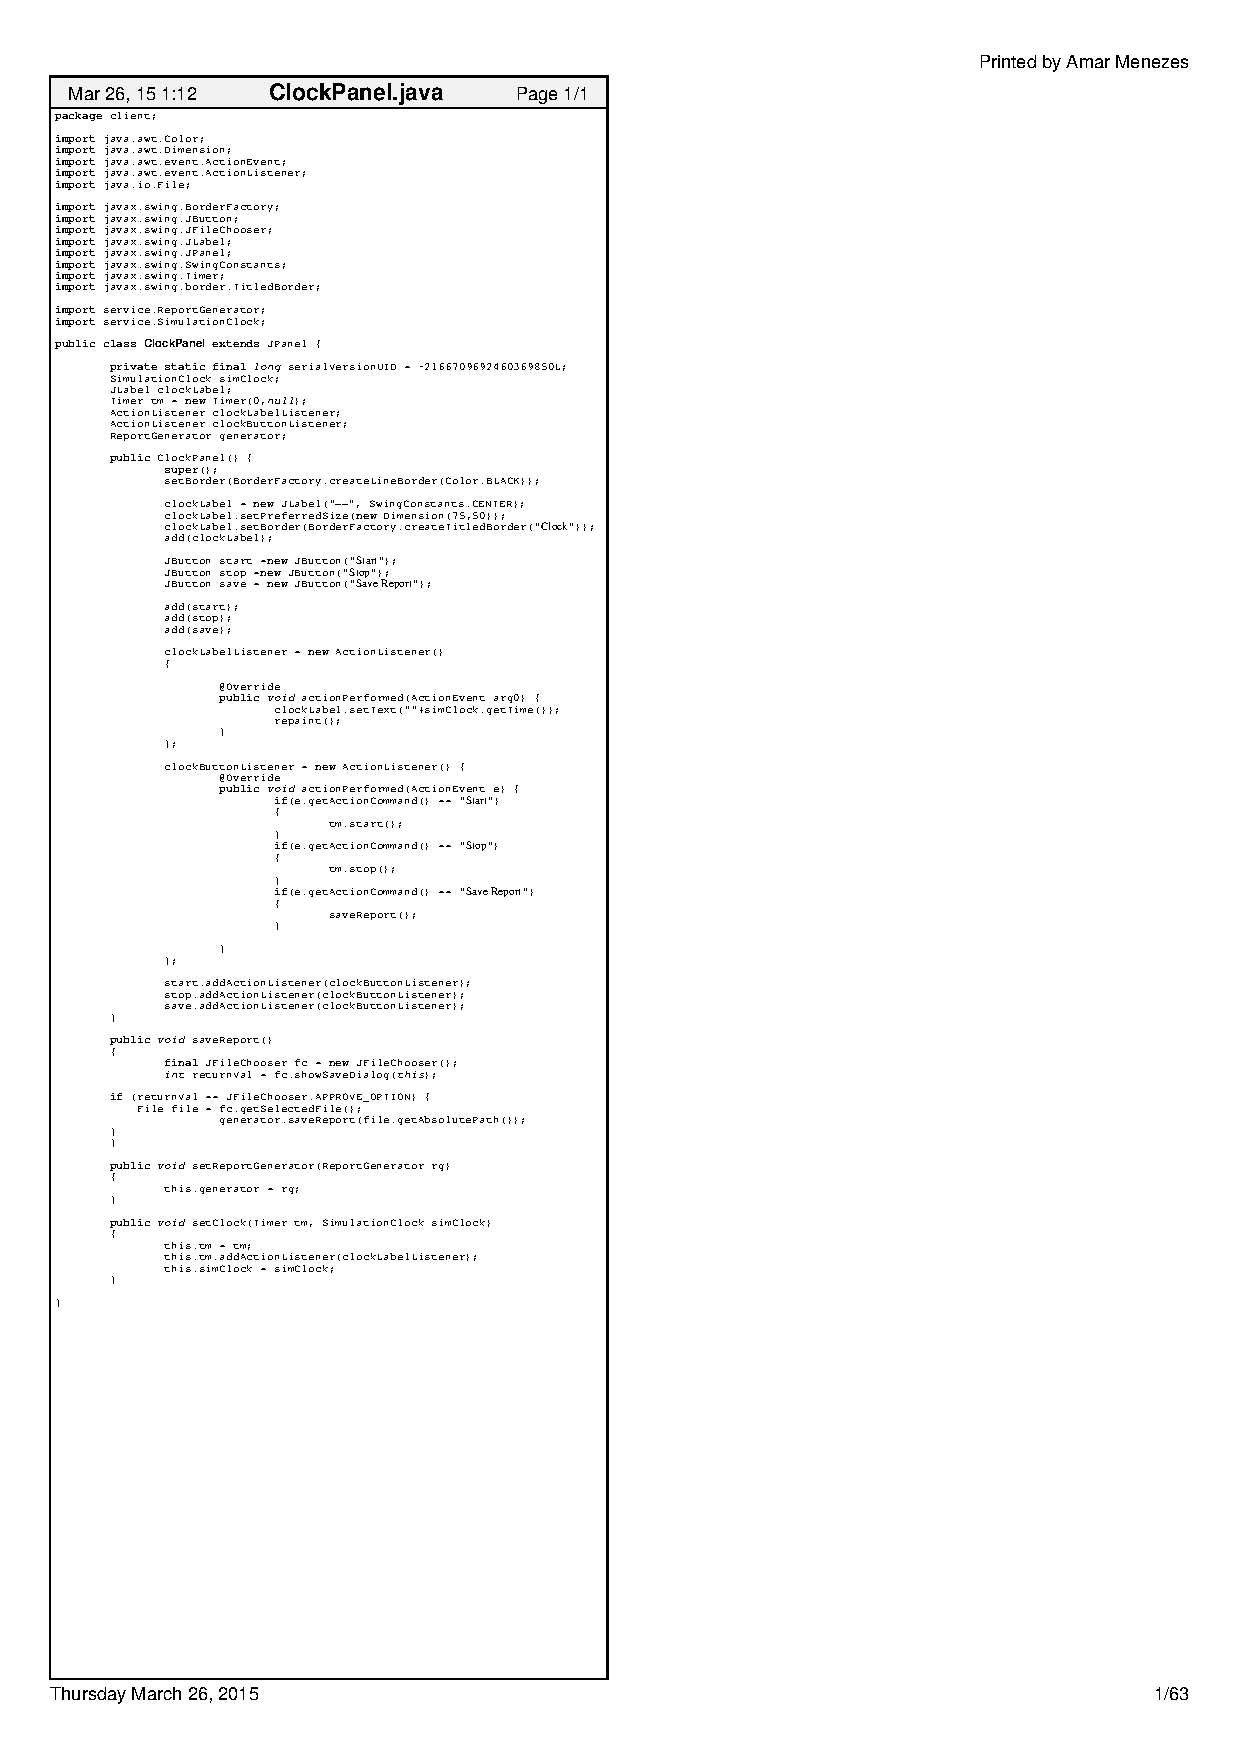
\includepdf[pages=-]{./files/TrafficSimSourceCode.pdf}


\end{document}